\section{二次函数与一元二次方程、不等式}

本节要点:
\begin{itemize}
    \item 从基本不等式深刻理解二次函数的最值。
\end{itemize}

~

虽然二次函数的标准形式为$y=ax^2+bx+c$,但以下方式更能说明二次函数:
\[
y=a\left( x+b \right) ^2+c
\]
\begin{itemize}
    \item 首先,通过$a$变换开口大小和方向,$a$越小开口越宽大,$a>0$开口向上;
    \item 然后,通过$b$进行沿{\it x}轴的平移,$b>0$左移;
    \item 最后,通过$c$进行沿{\it y}轴的平移,$c>0$上移。
\end{itemize}

\begin{figure}[h]
\centering
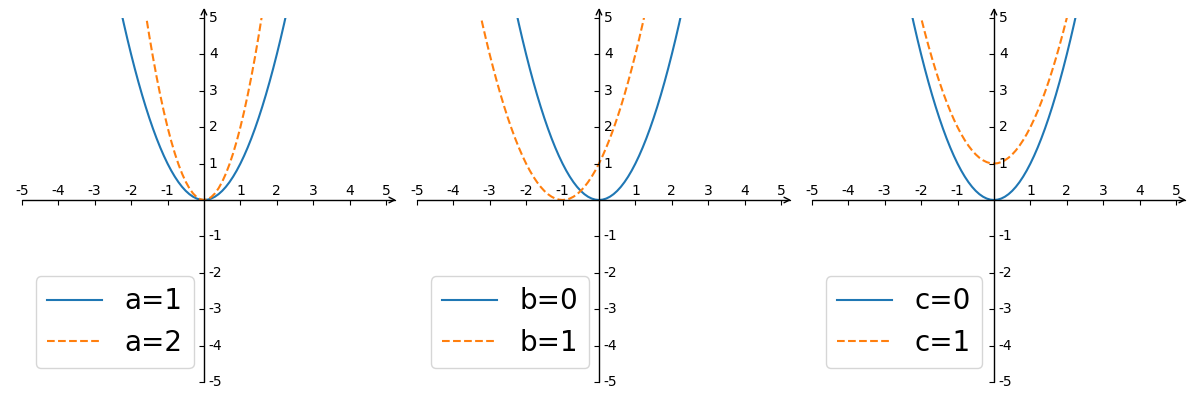
\includegraphics[height=4cm]{2.3-1.png}
\end{figure}

二次函数和基本不等式也可以相互推导。设某个变量$y$由$x,z$乘积决定,而$x,z$有关系$x+z=c$,其中 $c$为常数,于是:
\[
\begin{cases}
	y=x\cdot z\\
	x+z=c\\
\end{cases}\Rightarrow y=x\cdot \left( c-x \right)
\]
由基本不等式可得:
\[
y=x\cdot \left( c-x \right) \leqslant \left[ \frac{x+\left( c-x \right)}{2} \right] ^2=\frac{c^2}{4}
\]
用二次函数的方法:
\[
y=-x^2+cx
\]
当且仅当$x=\frac{c}{2}$时,$y$取最大值$y_{\max}=\frac{c^2}{4}$。

\begin{tcolorbox}
当两个变量的和为常量时,它们的积有最大值,这点从基本不等式和二次函数都能得到一样的结果。
\end{tcolorbox}

\begin{tcolorbox}
工程中,我们通常为最值构造一个二次函数$y=f\left( x_1,x_2 \right) $,用$ax_1+bx_2=c$作为两个变量的约束条件,得到一个二次函数,最终可求解最值。
\end{tcolorbox}

~

\begin{example}[综合运用4,难度:$\star $]
一名同学以初速度$v_0=12\mathrm{m}/\mathrm{s}$竖直向上抛一排球,排球能够在抛出点2m以上大的位置最多停留多长时间(精确到0.01s)?
\end{example}

\begin{figure}[h]
\centering
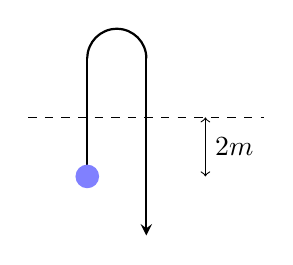
\begin{tikzpicture}[line join=round, scale=0.75]
\draw[thick] (0,0)--(0,2);
\draw[thick] (1,2) arc [start angle=0,end angle=180,radius=0.5cm];
\draw[thick,-stealth] (1,2)--(1,-1);
\fill[blue!50!white] (0,0) circle (2mm);
\draw[dashed] (-1,1)--(3,1);
\draw[<->] (2,1)--(2,0);
\coordinate[label=right:{$2m$}] (t) at (2,0.5);
\end{tikzpicture}
\end{figure}

解:

排球距抛出点高度和时间的关系如下:
\[
h=v_0t-\frac{1}{2}gt^2
\]
带入$v_0=12\mathrm{m}/\mathrm{s},g=10\mathrm{m}/\mathrm{s}^2,h\geqslant 2\mathrm{m}$得:
\[
12t-5t^2\geqslant 2
\]
令$5t^2-12t+2=0$,解得$t_{1,2}=\frac{12\pm \sqrt{12^2-4\cdot 5\cdot 2}}{2\cdot 5}=2.220 \,\, \mathrm{or} \,\, 0.180$,于是停留时间为$t=2.220-0.180=2.04\mathrm{s}$。

\begin{tcolorbox}
本题看似难,其实一点不难,物理问题已经转化为数学问题,剩下的就是体力活。
\end{tcolorbox}




